%!TEX root = proj_report_outline.tex

\chapter{Web Application Design}\label{C:design_web}

In this Chapter the design of the PitchHub prototype is discussed. Important aspects such as the user stories and UI design artefacts are explored. Finally, architectural decisions are reflected upon.

\section{User Stories}

The principal function of PitchHub is to facilitate collaboration in the innovation community, this is reflected in requirement D1. To achieve this, it is necessary to understand exactly what online collaboration in the innovation community looks like. An investigation into this found no existing works. 

As such the design of PitchHub began with specifying the fundamentals of online innovation collaboration in user stories. To do this, each user story captured a desired behaviour by identifying the behaviour's corresponding `who', `what', and `why' attributes. An example user story capturing \textit{Create Pitch Card} behaviour is as follows:

\begin{verbatim}
	  As a user, I want to create a Pitch Card so that the community and I may 
	  collaborate to find a solution	
\end{verbatim}

To unpack on this example, the `who' is a user, the `what' is the ability create Pitch Cards, and the `why' is the desire of finding a solution through collaboration.
So from these user stories not only is the behaviour captured but also relevant expectations of state. To continue using the above example, it can be discerned that once the user has posted a Pitch Card there is an expectation that other users will be able to see it and also interact with it `to find a solution'. 

User stories, such as the following, were also used to introduce the different actors involved in the community:

\begin{verbatim}
    As an initiator, I want to see who has viewed my content so that I 
    have an account of it's dissemination
\end{verbatim}

In this example, the initiator is the `who' and the expectation is that they have extra functionality which enables them to audit who has seen the Pitch Card they initiated. This notion of variable functionality/visibility levels given your relationship to the content is central to the innovation collaboration process. To ensure the accuracy of these user stories, specification was done in collaboration with Callaghan Innovation. 

To have a complete understanding of the functionality required by PitchHub, user stories were used to describe all desired behaviour, ranging from sign-up to content scoping (as per requirement D2.1). These user stories are found in Appendix \ref{A:user_stories}.


\section{UI Design}
A well-designed user interface drives user behaviour. Given PitchHub's aim of facilitating collaboration behaviour it is advantageous to have it also drive it. Specifically the behaviour aimed to be driven is those found in requirements D1, D2.1, and D2.2. To do this, the behaviour captured in the user stories were embraced in the content templates and wire frames created to guide the final UI design. An example content template for the Pitch Card page is displayed in Figure \ref{fig:content_template}.
The creation of content templates for each page were the first step in UI design. Content templates were used as they place emphasis on the narrative of each page being designed first before the visual elements, thus prioritising the fundamentals. Ultimately, through content templates each page is deconstructed into: who the target audience is, what the page's purpose is, and what the context is.

\begin{figure}[ht]
    \centering
    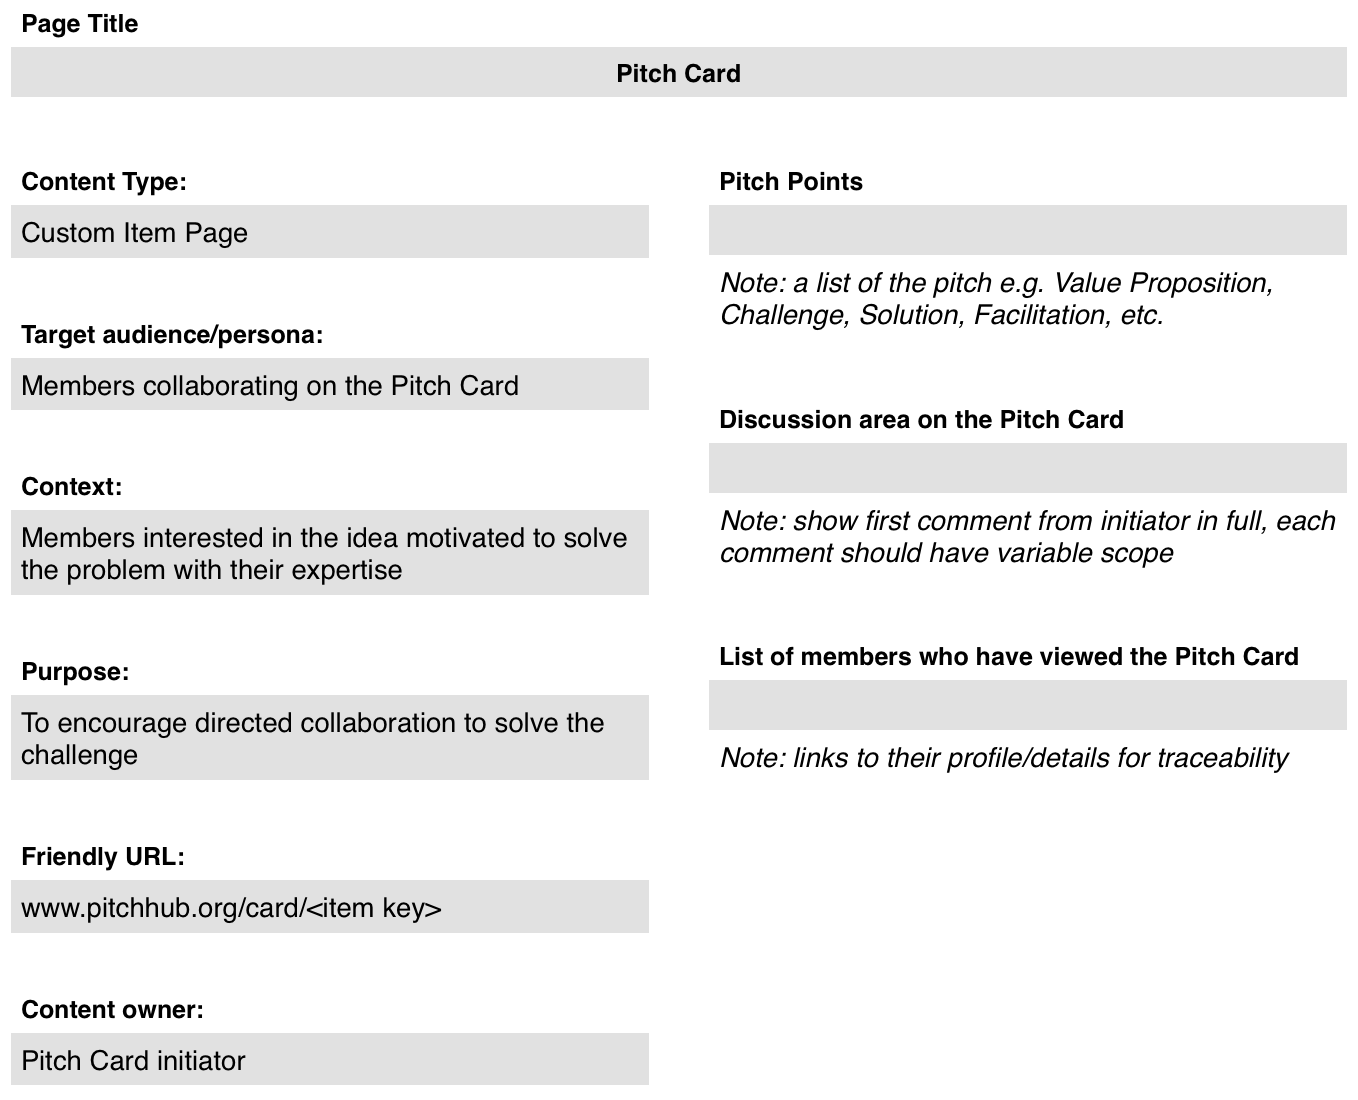
\includegraphics[width=0.6\textwidth]{show_pitch_card_content_template}
    \caption{Content template for the ``Show Pitch Card'' page. The content template is organised into two sections: supporting information and metadata on the left, and page content on the right. A larger version is displayed in Appendix \ref{A:content_template}.}
    \label{fig:content_template}
\end{figure}

Wire frames were then used to plan the layout of each page. This process solely focused on the layout and visual design of each page rather than determining the content (already specified in the content templates). For example, the Pitch Card page wire frame, Figure \ref{fig:wire_frame}, simply visualises the content specified in it's content template, Figure \ref{fig:content_template}.

There exist only minor differences between the wire frames created and the final implementation. An example difference is the lack of ``Make Suggestion'' button. This button has been removed as the final implementation enables users to make suggestions on the Pitch Points through in-line editing (see Figure \ref{fig:show_pitch_card}). Not only is this regarded as a more natural interaction but also a behaviour driver. Making a suggestion in-line in the context of the Pitch Card is designed to encourage suggestions that are considered in the theme of the Pitch Card as a whole.

Wire frames were also used to guide the design of PitchHub on mobile form factors. Given the increasing trend of mobile browser usage, now accounting for a third of web traffic \cite{Mobile_rise:online} it is important that PitchHub features mobile support. The wide range of mobile sizes made it necessary for the layout to have a responsive design. Fig. \ref{fig:wire_frame_mobile} demonstrates the dashboard view's design for the mobile size. In this size the view utilises a list design whereas the the grid design is used for desktop sizes.

\begin{figure}[ht]
  \begin{subfigure}[t]{.45\textwidth}
  \centering
    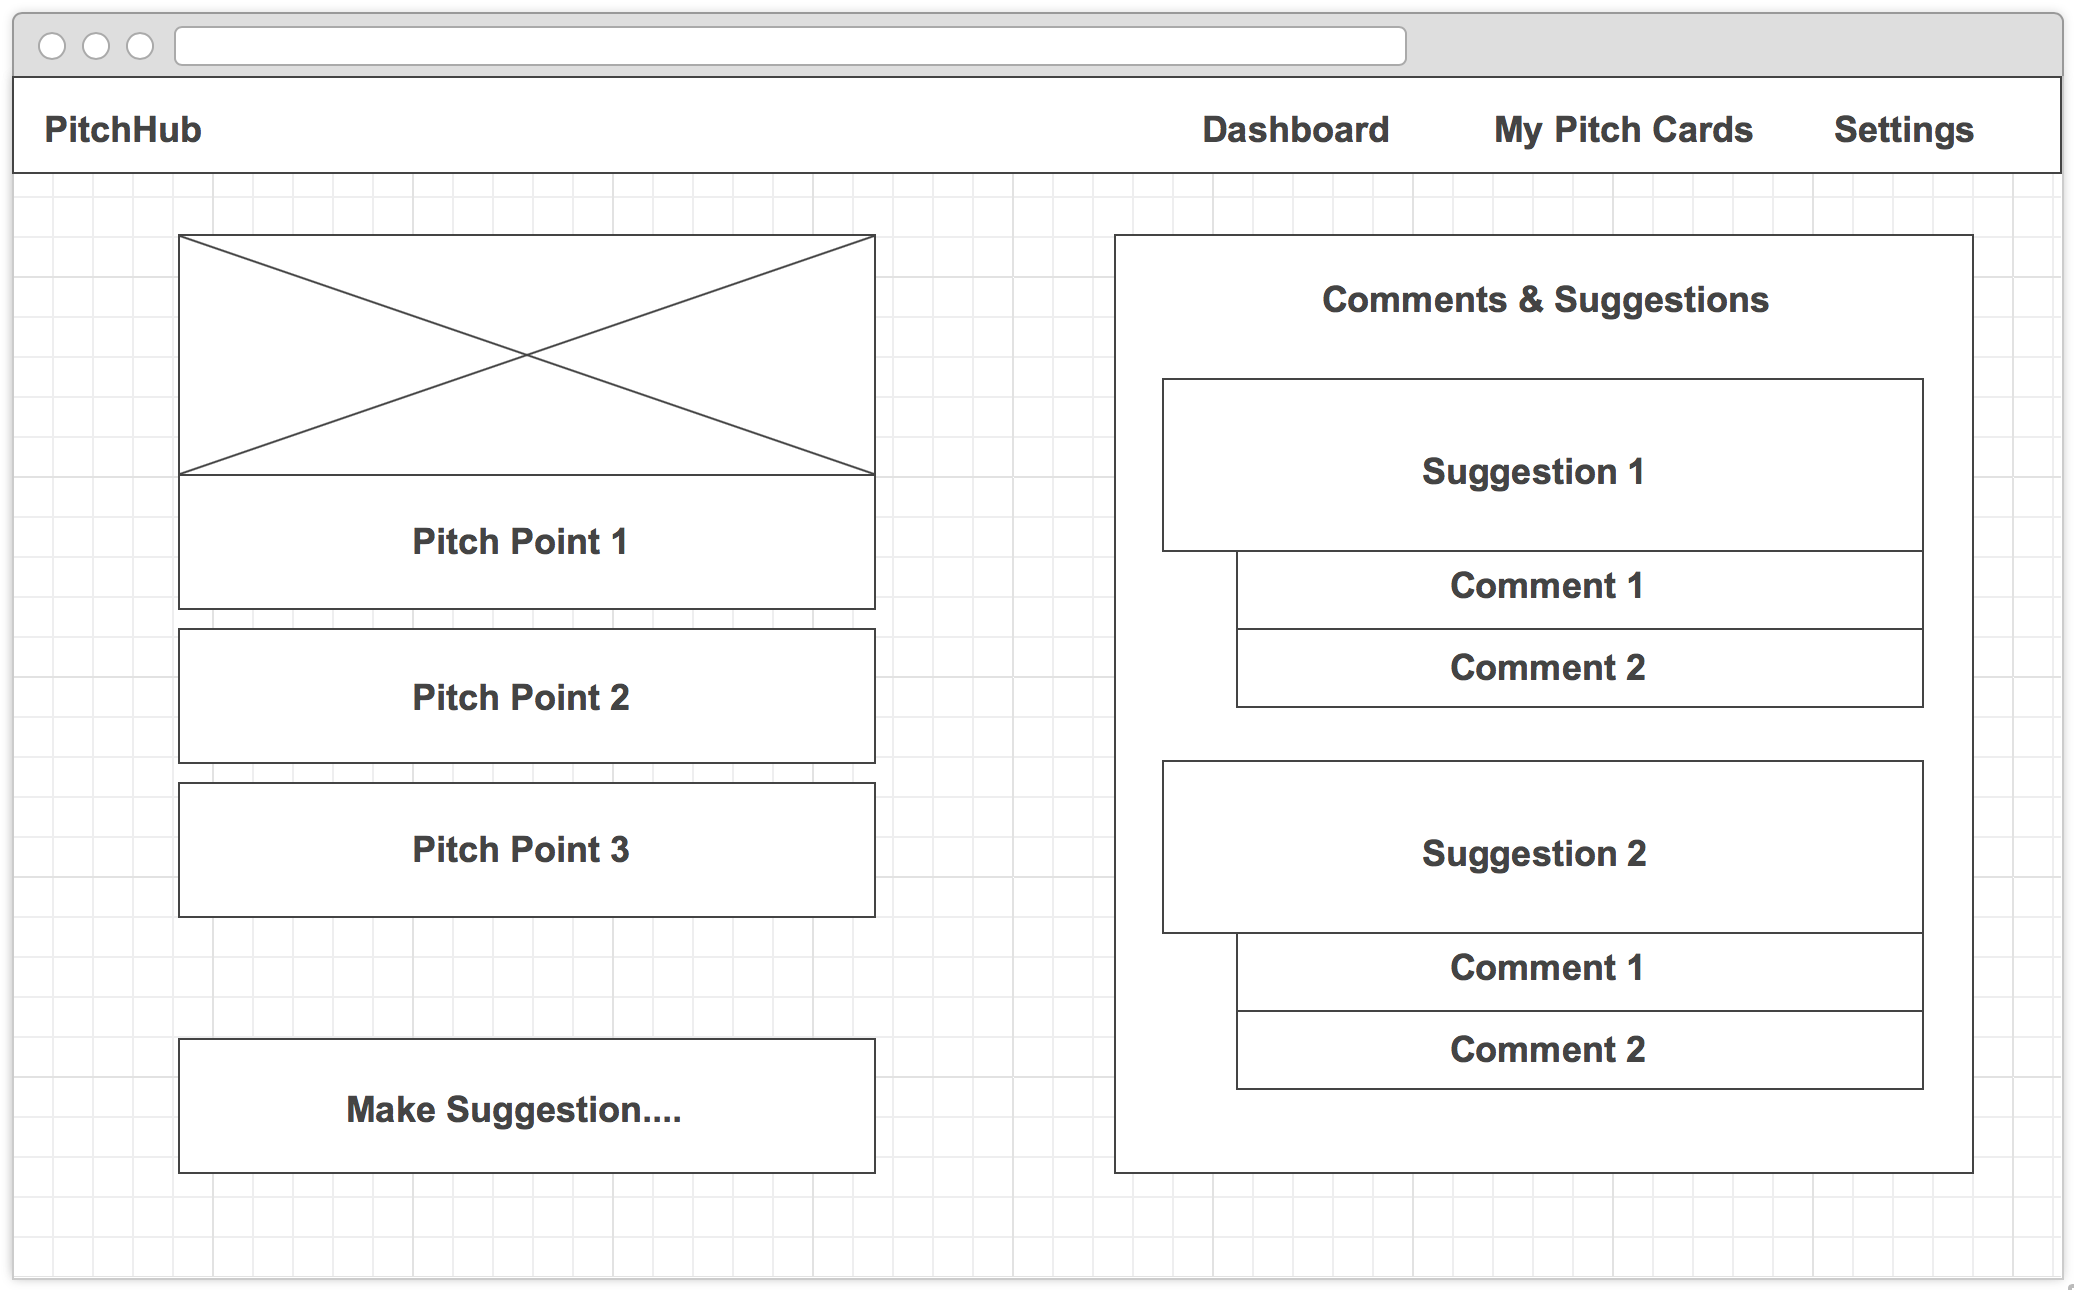
\includegraphics[width=1\textwidth]{wire_frame}
    \caption{Wire frame of the ``Show Pitch Card'' page. The primary features are the Pitch Points on the left, and suggestions with comments on the right. Users can contribute suggestions by clicking the ``Make Suggestion'' button. See Figure \ref{fig:show_pitch_card} for final implementation.}
    \label{fig:wire_frame}
  \end{subfigure}\hfill
  \begin{subfigure}[t]{.45\textwidth}
  \centering
    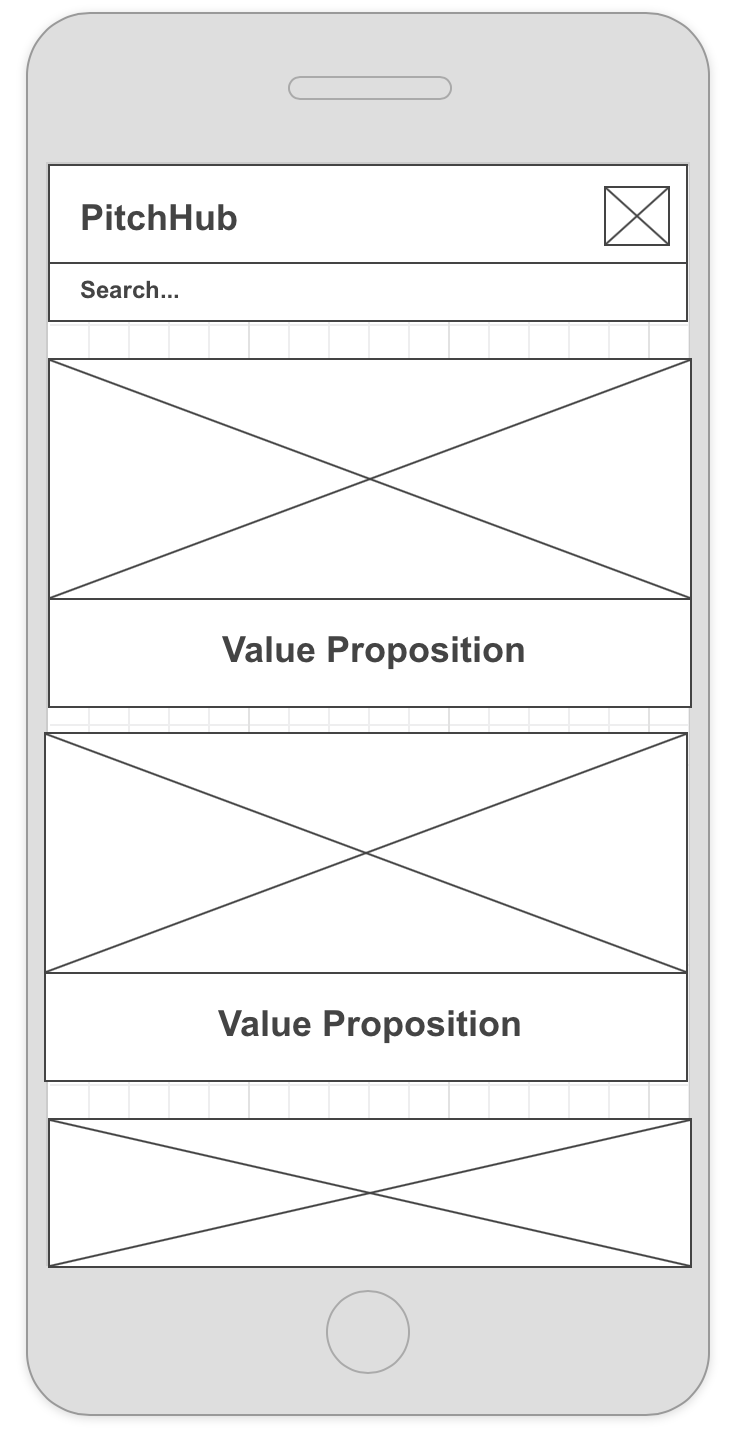
\includegraphics[width=.4\textwidth]{wire_frame_dashboard_mobile}
    \caption{Wire frame of the ``Dashboard'' page on a mobile. The primary features are the concatenated Pitch Cards and the search function. See Figure \ref{fig:dashboard_mobile_pitchhub} for final implementation.}
    \label{fig:wire_frame_mobile}
  \end{subfigure}
  \caption{Example wire frames used to guide final implementation.}
\end{figure}

\section{Architecture}

A key aspect of PitchHub's distributed architecture design is separation of concerns (SoC). Systems that embody SoC generally use encapsulation to achieve modularity. SoC was identified as a fundamental feature for aiding PitchHub's extensibility, per requirement D3. PitchHub's SoC is primarily achieved through the adoption of the three-tier architecture, consisting of the following: 

\begin{description}
  \item[presentation tier] communicates user interaction to the application tier and displays the content in a structured view using HTML and SASS. AJAX has been leveraged so that interaction with the application tier can occur without reloading the entire page.
  \item[application tier] performs business logic and responds to user interaction. To simplify the request life-cycle, SoC has been applied further with the MVC pattern. The SoC in this tier enables complex sets of interactions to be standardised, conforming to conventions that are well defined and that can be easily be understood \cite{leff2001web}.
  \item[data tier] persists application data in a distributed configuration. The data intensive nature of PitchHub means that it can improve it's performance through spreading the data and processing logic among nodes. This kind of approach is known as a shared nothing architecture \cite{stonebraker1986case}, prevalent in NoSQL systems. The \textit{n} number of databases shown in Figure \ref{fig:architecture_1} act as the secret keepers for the database security security scheme discussed in Chapter \ref{C:threshholdSecurity}.
\end{description}

Ultimately, through this SoC PitchHub can switch out modules without affecting neighbouring tiers given they conform to the same interface. Or if changes to the interface are required then only the neighbouring tier is needed to be changed. 

\begin{figure}[ht]
    \centering
    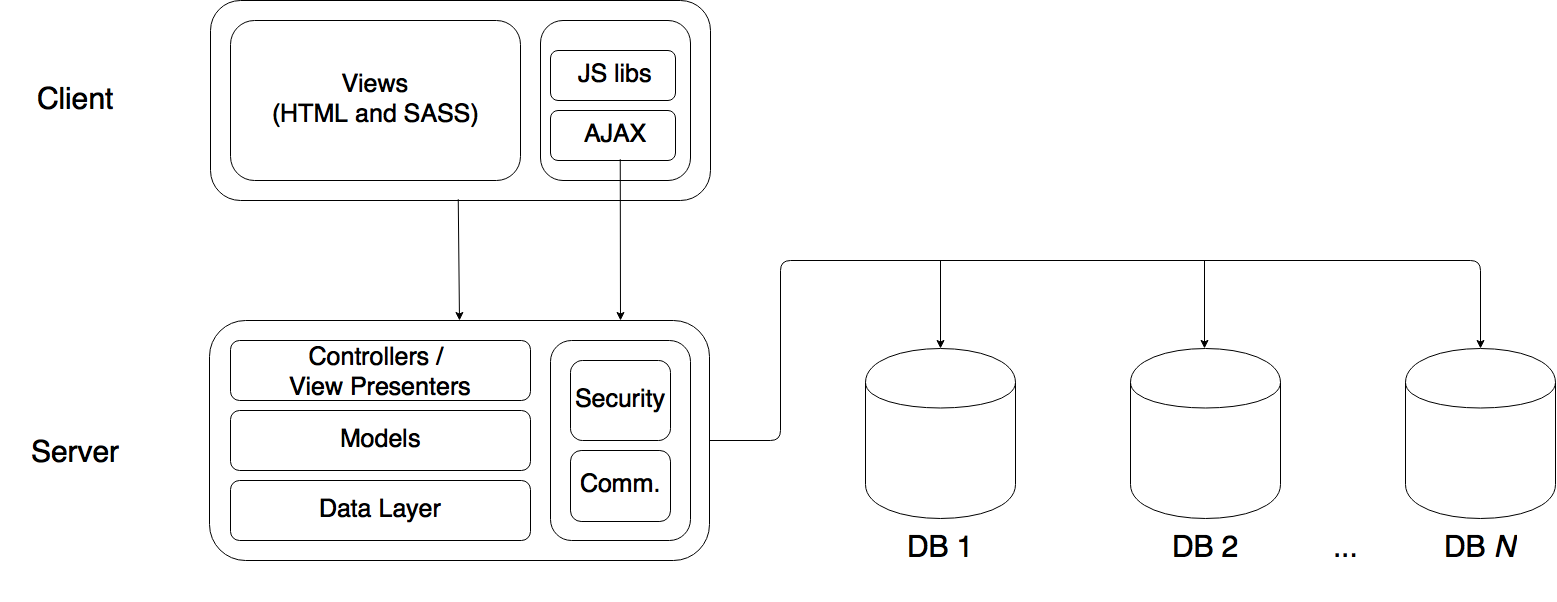
\includegraphics[width=1\textwidth]{initial_architecture}
    \caption{The 3-tier architecture designed for PitchHub. Key attributes to note are: the separation of concerns (for requirement D3) and the variable number of \textit{n} databases.}
    \label{fig:architecture_1}
\end{figure}

\section{System Model}\label{S:systemModel}

Fig \ref{fig:class_diagram} displays the system model in a class diagram. The functionality to support requirement D2.1's privacy controls is captured through the Pitch Card and Comment classes' relationship with the DisclosureScope class. This DisclosureScope class essentially filters out any associated content if a viewer not meet it's requirements. With Pitch Cards this is fairly simple: an initiator sets the scope as they create the Pitch Card, and only those who satisfy the scope can see the Pitch Card.

This scoping works similarly with Comments and Suggestions on Pitch Points however business logic ensures that the  scoping can only be set to an equivalent or more restrictive level than that specified in the Pitch Card being commented/suggested on. An example of this is where an initiator set's the content scope to `Members', so only members of the PitchHub can view the idea, if a user were to contribute a suggestion on a Pitch Point this suggestion can only be scoped as `Members' or any level which is more restrictive, they cannot however set it to `Public'. 

To make the scoping functionality more extensible it has been designed with the strategy pattern, see Figure \ref{fig:class_diagram}.
 
\begin{sidewaysfigure}[ht]
    \centering
    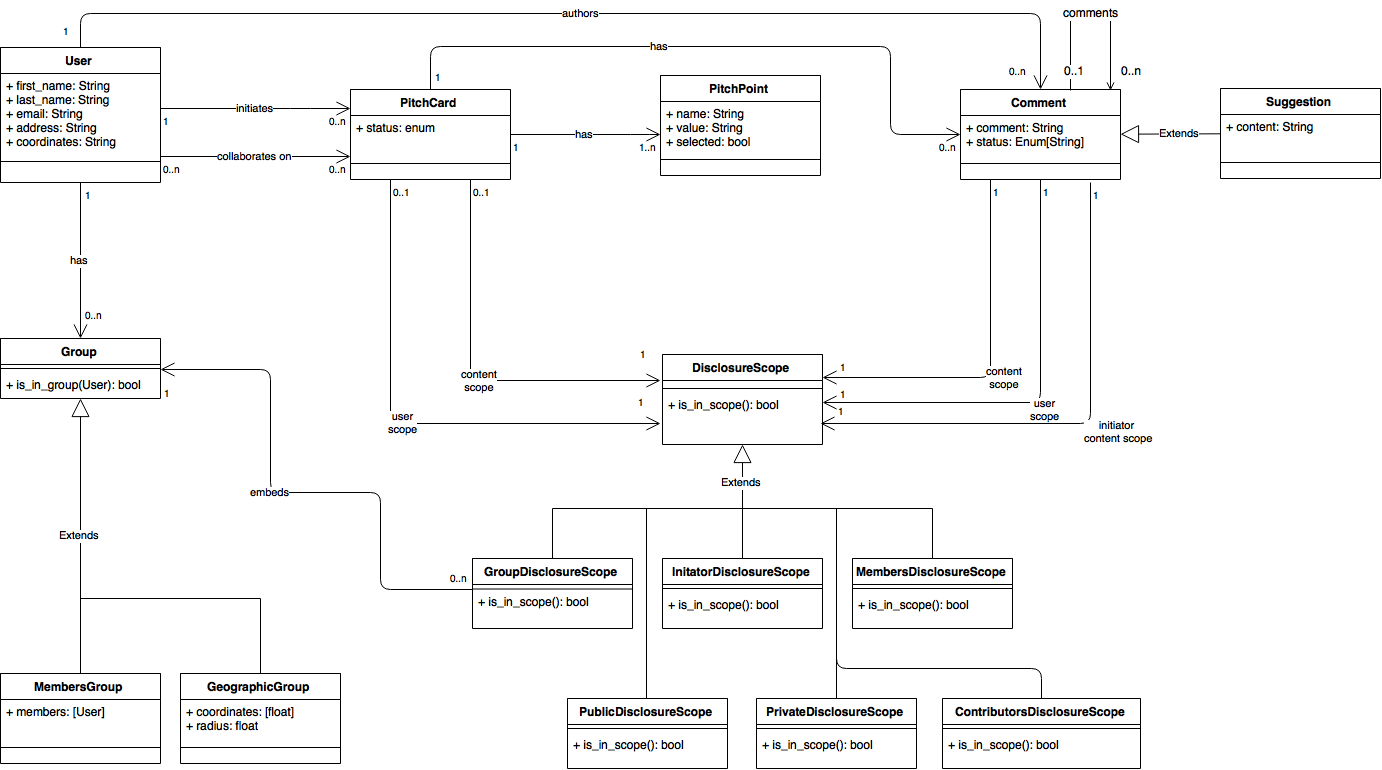
\includegraphics[width=1\textwidth]{class_diagram}
    \caption{PitchHub's system structure as represented in a class diagram. Of note is the Pitch Card and Comment classes and their relationship to the DisclosureScopes. This relationship describes the Pitch Card and Comment classes ability to scope the visibility of their content. (NB: Some attributes were left out for the sake of brevity e.g. Pitch Cards have an `images' attribute)}
    \label{fig:class_diagram}
\end{sidewaysfigure}

\section{Technology}

The overall performance and quality of service of an application is deeply influenced by the frameworks and infrastructure it is built upon. In this section both the framework and database selections are discussed in relation to quality of service attributes and more importantly the requirements identified in Chapter \ref{C:requirements}.

\subsection{Framework Selection}\label{SS:frameworkSelection}

Research was conducted on the web application frameworks available in effort to speed up the prototyping process. Ruby on Rails, Laravel, Django, MEAN and OpenSocial were identified as frameworks that could work in fulfilment of the requirements specified. Ultimately the choice of frameworks was between Ruby on Rails and OpenSocial as these were identified as being the most accessible. Ruby on Rails is an open source framework that embraces RESTful web service design and conforms to the MVC architecture. Of note, Ruby on Rails has a wealth of open-source secret sharing and functional testing libraries that are directly applicable to the requirements of this project. OpenSocial in contrast to Ruby on Rails is first and foremost a framework for creating social networks, and while PitchHub is not specifically a social network it's primary objective is to facilitate social interaction. Using OpenSocial would offer user authentication as well as messaging and posting functionality out of the box. 
\par
Of these frameworks Ruby on Rails was selected because of its vast open source library and elegant handling of complex user interaction flows. This decision results in a trade off in performance due to Ruby on Rails using Ruby and OpenSocial using Java. Even in the current versions of each language Java has a significant  performance advantage over Ruby \cite{Perfo1:online}. For a simple web application this generally would not be a concern, however the secret sharing component entails the use of encryption algorithms which are computationally expensive. This was concluded not to be a major issue as Ruby on Rails offers the ability to run JRuby which is Ruby executed atop the JVM. JRuby offers significantly improved performance and even allows native Java to be executed if necessary \cite{Jruby:online}.

\subsection{Database Selection}\label{SS:databaseSelection}

The choice of database has profound effects on requirements D4 and D5. The rise of NoSQL databases has been attributed to the increasing need for highly scalable and performant databases. Given this need in PitchHub, in addition to PostgreSQL (Postgres), the NoSQL databases MongoDB and Cassandra were also investigated.
\par
The nature of the Pitch Card data PitchHub is modelling is inherently hierarchical and heterogeneous. In PitchHub, each Pitch Card has a varying number of Pitch Points, and each Pitch Point also contains a number of interaction attributes. This data model naturally lends itself to the document model offered by MongoDB. Pitch Cards may be modelled in a single document with Pitch Point relations expressed via embedding. This has the additional benefit of being able to efficiently query the Pitch Cards.
\par
The case for using a relational database like Postgres is also motivated by the inherent nature of PitchHub's data. For example, each user is associated to the Pitch Cards they have initiated and contributed to, as well as the suggestions and comments they have offered on Pitch Cards. Unlike the internal model of Pitch Cards these relations are not well suited to being hierarchical as these relations have associations which are N:M rather than 1:1 or 1:N. Modelling these objects separately in tables and querying them through joins in the relational model is the ideal way to represent and query these relations.
\par
Ultimately both databases were decided to be used in PitchHub as part of the Threshold scheme (discussed in Section \ref{SS:diverse_secret_keepers}). MongoDB has been configured as the default database in the prototype. While Postgres has been used to diversify the Threshold scheme's secret keepers. MongoDB was chosen as the default because the Pitch Card data is well suited to MongoDB's data model and the use case flows which require joins at most only need one join operation. It was concluded that using MongoDB and performing manual joins within the application is not a major issue because of this. Also MongoDB's ability to scale horizontally easily without the expensive migrations characteristic of relational databases provides an edge over Postgres in meeting the scalability requirement.
